\documentclass[11pt]{article}
\usepackage[textwidth=18.0cm, textheight=23.0cm, top=2.0cm]{geometry}
\usepackage{pst-all}
\usepackage{amssymb}
\usepackage{tikz}
\usepackage{underscore}\begin{document}
\pagestyle{empty}


ClassName: \underline{\textbf{Class_03.2bp-43}}
\par
BinSize: \underline{\textbf{40 × 40}}
\par
ReduceSize: \underline{\textbf{40 × 40}}
\par
TypeNum: \underline{\textbf{96}}
\par
Num: \underline{\textbf{100}}
\par
OutS: \underline{\textbf{32000}}
\par
InS: \underline{\textbf{30525}}
\par
Rate: \underline{\textbf{0.954}}
\par
UB: \underline{\textbf{20}}
\par
LB0: \underline{\textbf{20}}
\par
LB: \underline{\textbf{20}}
\par
LBWithCut: \underline{\textbf{20}}
\par
NodeCut: \underline{\textbf{0}}
\par
ExtendedNodeCnt: \underline{\textbf{1}}
\par
GenNodeCnt: \underline{\textbf{1}}
\par
PrimalNode: \underline{\textbf{0}}
\par
ColumnCount: \underline{\textbf{20}}
\par
TotalCutCount: \underline{\textbf{0}}
\par
RootCutCount: \underline{\textbf{0}}
\par
LPSolverCnt: \underline{\textbf{1}}
\par
PricingSolverCnt: \underline{\textbf{0}}
\par
BranchAndBoundNum: \underline{\textbf{1}}
\par
isOpt: \underline{\textbf{true}}
\par
TimeOnInitSolution: \underline{\textbf{600.000 s}}
\par
TimeOnPrimal: \underline{\textbf{0.000 s}}
\par
TimeOnPricing: \underline{\textbf{0.000 s}}
\par
TimeOnRmp: \underline{\textbf{0.062 s}}
\par
TotalTime: \underline{\textbf{600.344 s}}
\par
\newpage


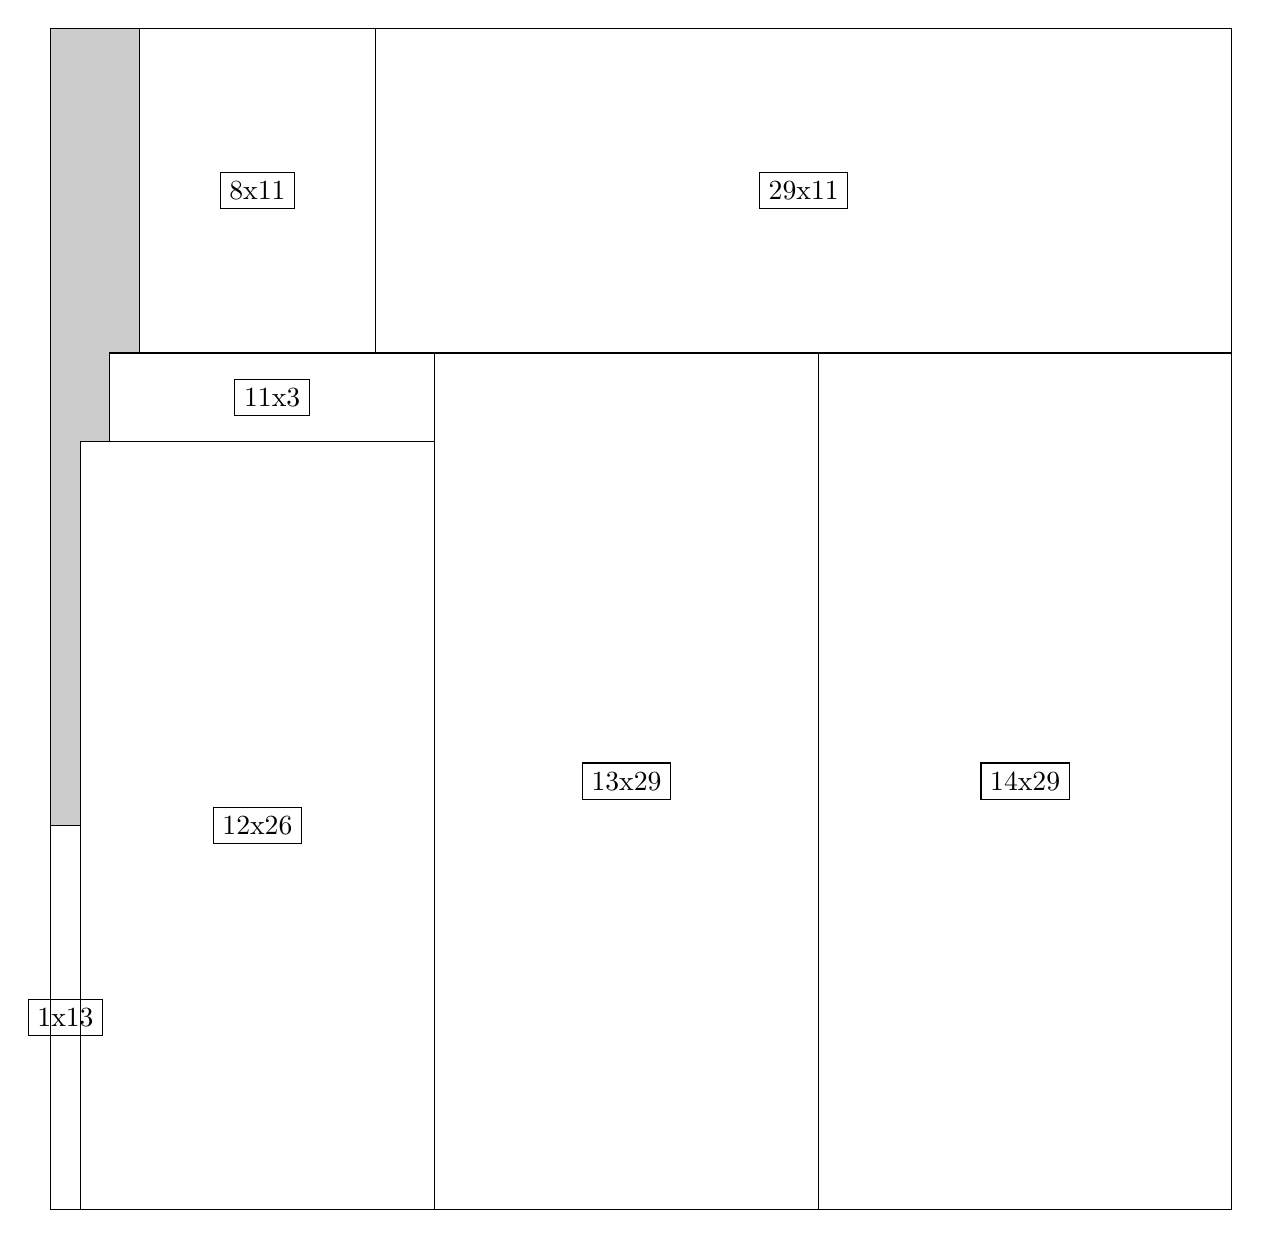
\begin{tikzpicture}[shorten >=1pt,scale=1.0,every node/.style={scale=1.0},->]
\tikzstyle{vertex}=[circle,fill=black!25,minimum size=14pt,inner sep=0pt]
\filldraw[fill=gray!40!white, draw=black] (0,0) rectangle (15.0,15.0);
\foreach \name/\x/\y/\w/\h in {14x29/9.75/0.0/5.25/10.875,13x29/4.875/0.0/4.875/10.875,12x26/0.375/0.0/4.5/9.75,1x13/0.0/0.0/0.375/4.875,11x3/0.75/9.75/4.125/1.125,29x11/4.125/10.875/10.875/4.125,8x11/1.125/10.875/3.0/4.125}
\filldraw[fill=white!40!white, draw=black] (\x,\y) rectangle node[draw] (\name) {\name} ++(\w,\h);
\end{tikzpicture}


w =14 , h =29 , x =26 , y =0 , v =406
\par
w =13 , h =29 , x =13 , y =0 , v =377
\par
w =12 , h =26 , x =1 , y =0 , v =312
\par
w =1 , h =13 , x =0 , y =0 , v =13
\par
w =11 , h =3 , x =2 , y =26 , v =33
\par
w =29 , h =11 , x =11 , y =29 , v =319
\par
w =8 , h =11 , x =3 , y =29 , v =88
\par
\newpage


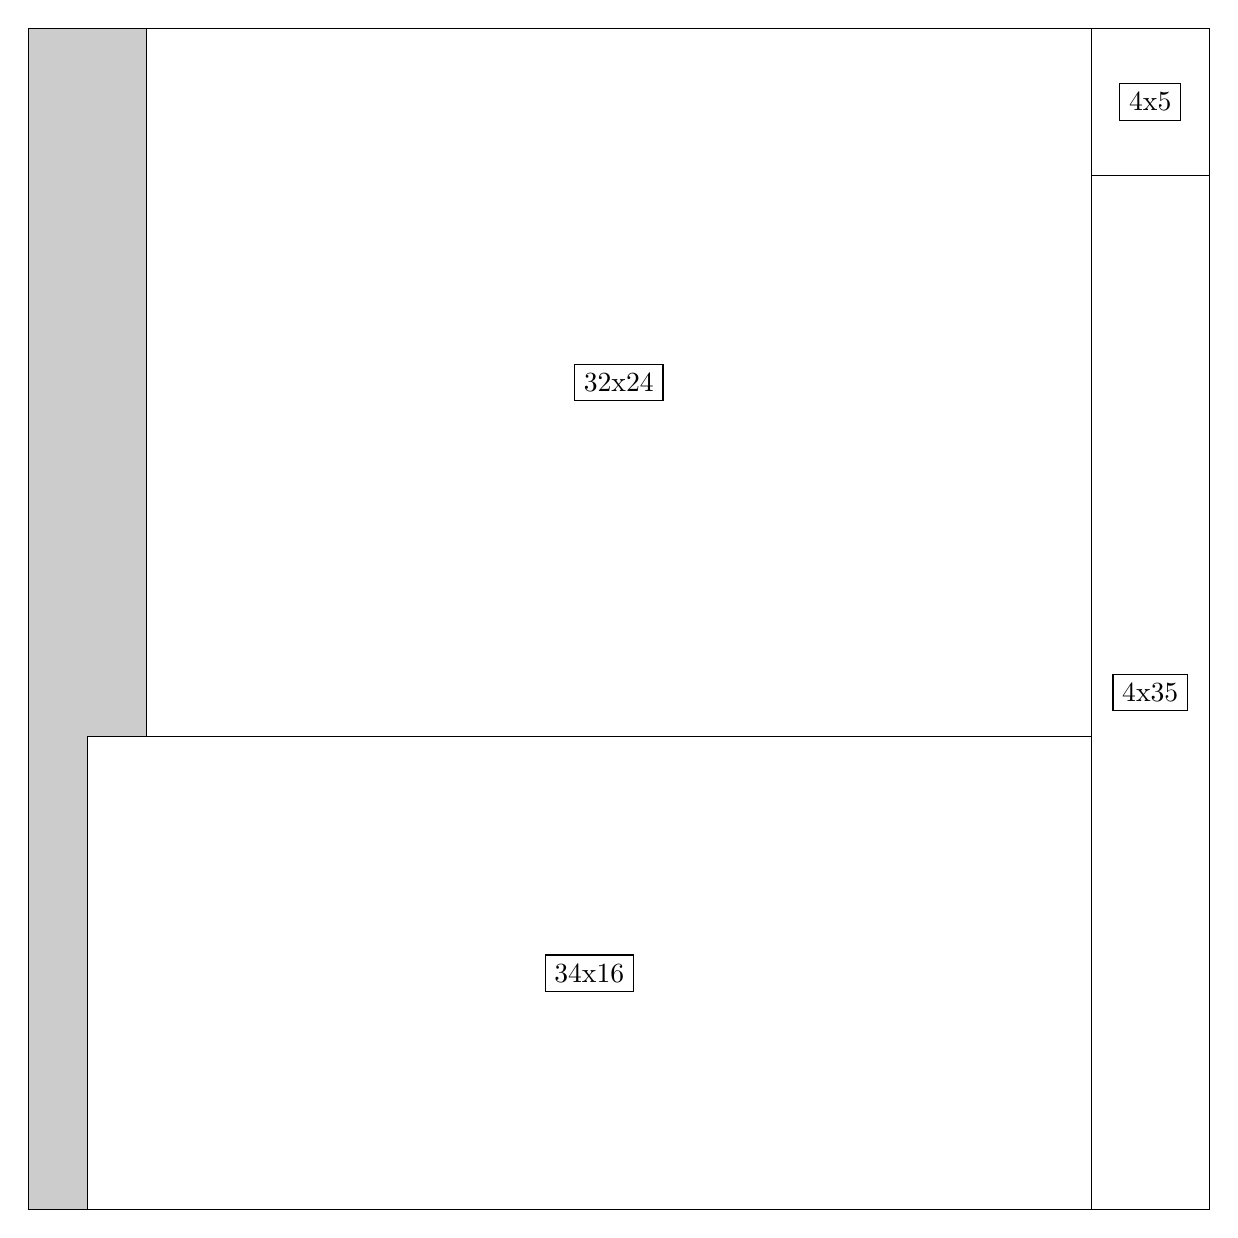
\begin{tikzpicture}[shorten >=1pt,scale=1.0,every node/.style={scale=1.0},->]
\tikzstyle{vertex}=[circle,fill=black!25,minimum size=14pt,inner sep=0pt]
\filldraw[fill=gray!40!white, draw=black] (0,0) rectangle (15.0,15.0);
\foreach \name/\x/\y/\w/\h in {4x35/13.5/0.0/1.5/13.125,4x5/13.5/13.125/1.5/1.875,34x16/0.75/0.0/12.75/6.0,32x24/1.5/6.0/12.0/9.0}
\filldraw[fill=white!40!white, draw=black] (\x,\y) rectangle node[draw] (\name) {\name} ++(\w,\h);
\end{tikzpicture}


w =4 , h =35 , x =36 , y =0 , v =140
\par
w =4 , h =5 , x =36 , y =35 , v =20
\par
w =34 , h =16 , x =2 , y =0 , v =544
\par
w =32 , h =24 , x =4 , y =16 , v =768
\par
\newpage


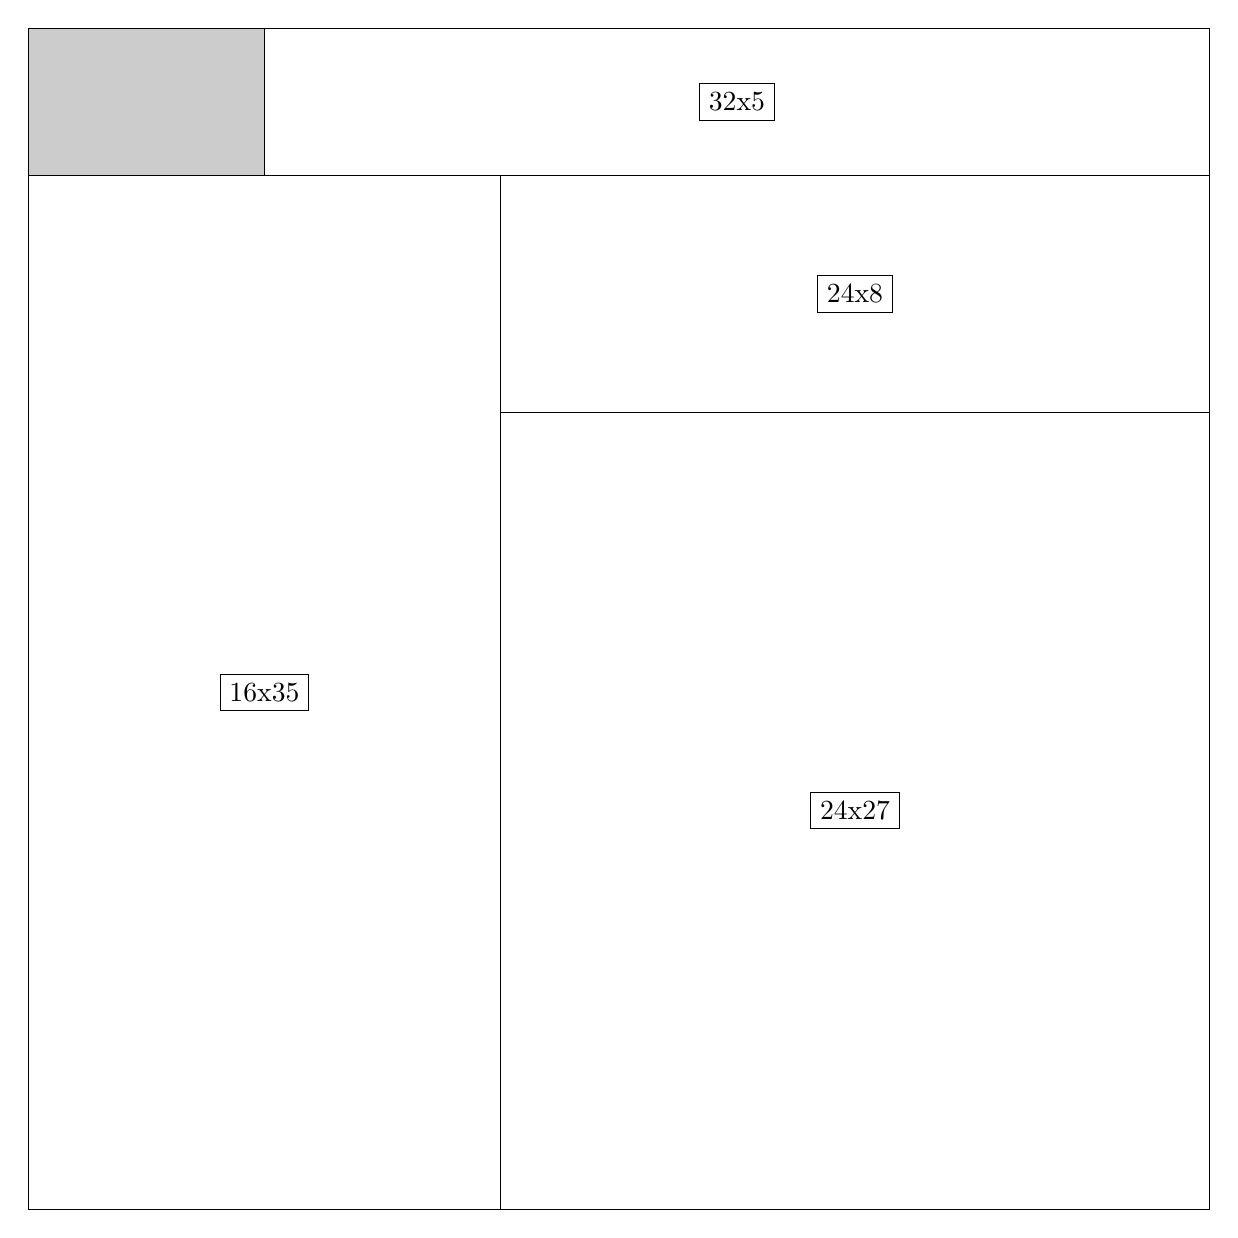
\begin{tikzpicture}[shorten >=1pt,scale=1.0,every node/.style={scale=1.0},->]
\tikzstyle{vertex}=[circle,fill=black!25,minimum size=14pt,inner sep=0pt]
\filldraw[fill=gray!40!white, draw=black] (0,0) rectangle (15.0,15.0);
\foreach \name/\x/\y/\w/\h in {24x27/6.0/0.0/9.0/10.125,24x8/6.0/10.125/9.0/3.0,16x35/0.0/0.0/6.0/13.125,32x5/3.0/13.125/12.0/1.875}
\filldraw[fill=white!40!white, draw=black] (\x,\y) rectangle node[draw] (\name) {\name} ++(\w,\h);
\end{tikzpicture}


w =24 , h =27 , x =16 , y =0 , v =648
\par
w =24 , h =8 , x =16 , y =27 , v =192
\par
w =16 , h =35 , x =0 , y =0 , v =560
\par
w =32 , h =5 , x =8 , y =35 , v =160
\par
\newpage


\begin{tikzpicture}[shorten >=1pt,scale=1.0,every node/.style={scale=1.0},->]
\tikzstyle{vertex}=[circle,fill=black!25,minimum size=14pt,inner sep=0pt]
\filldraw[fill=gray!40!white, draw=black] (0,0) rectangle (15.0,15.0);
\foreach \name/\x/\y/\w/\h in {15x32/9.375/0.0/5.625/12.0,15x8/9.375/12.0/5.625/3.0,25x14/0.0/0.0/9.375/5.25,22x21/1.125/5.25/8.25/7.875,3x19/0.0/5.25/1.125/7.125,24x5/0.375/13.125/9.0/1.875}
\filldraw[fill=white!40!white, draw=black] (\x,\y) rectangle node[draw] (\name) {\name} ++(\w,\h);
\end{tikzpicture}


w =15 , h =32 , x =25 , y =0 , v =480
\par
w =15 , h =8 , x =25 , y =32 , v =120
\par
w =25 , h =14 , x =0 , y =0 , v =350
\par
w =22 , h =21 , x =3 , y =14 , v =462
\par
w =3 , h =19 , x =0 , y =14 , v =57
\par
w =24 , h =5 , x =1 , y =35 , v =120
\par
\newpage


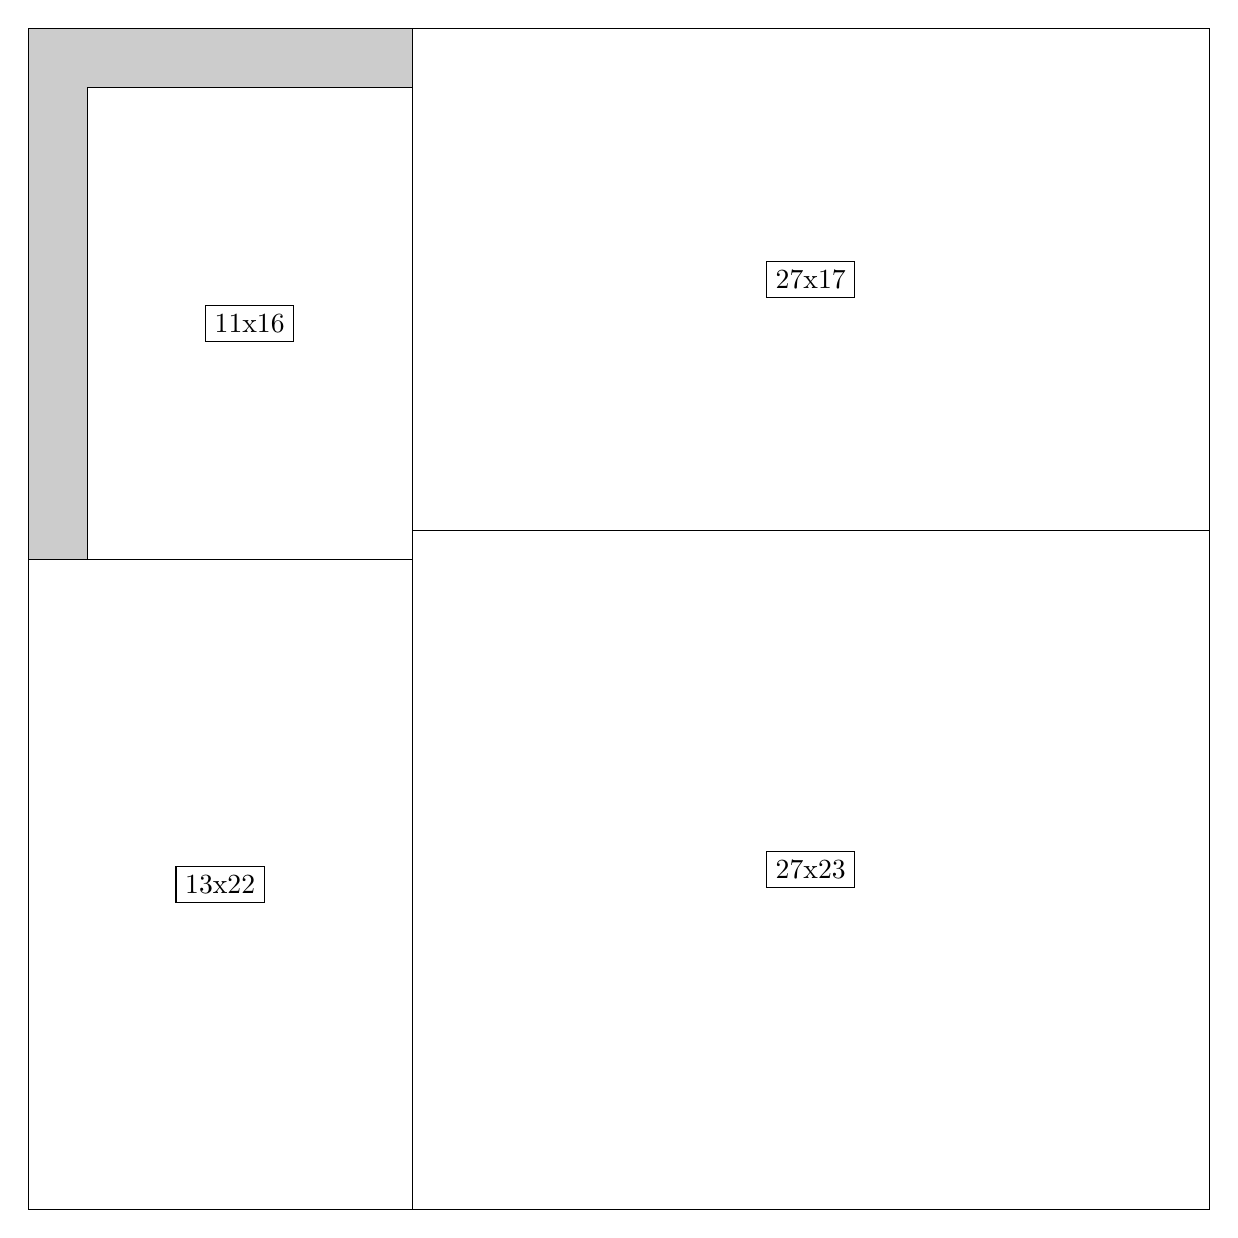
\begin{tikzpicture}[shorten >=1pt,scale=1.0,every node/.style={scale=1.0},->]
\tikzstyle{vertex}=[circle,fill=black!25,minimum size=14pt,inner sep=0pt]
\filldraw[fill=gray!40!white, draw=black] (0,0) rectangle (15.0,15.0);
\foreach \name/\x/\y/\w/\h in {27x23/4.875/0.0/10.125/8.625,27x17/4.875/8.625/10.125/6.375,13x22/0.0/0.0/4.875/8.25,11x16/0.75/8.25/4.125/6.0}
\filldraw[fill=white!40!white, draw=black] (\x,\y) rectangle node[draw] (\name) {\name} ++(\w,\h);
\end{tikzpicture}


w =27 , h =23 , x =13 , y =0 , v =621
\par
w =27 , h =17 , x =13 , y =23 , v =459
\par
w =13 , h =22 , x =0 , y =0 , v =286
\par
w =11 , h =16 , x =2 , y =22 , v =176
\par
\newpage


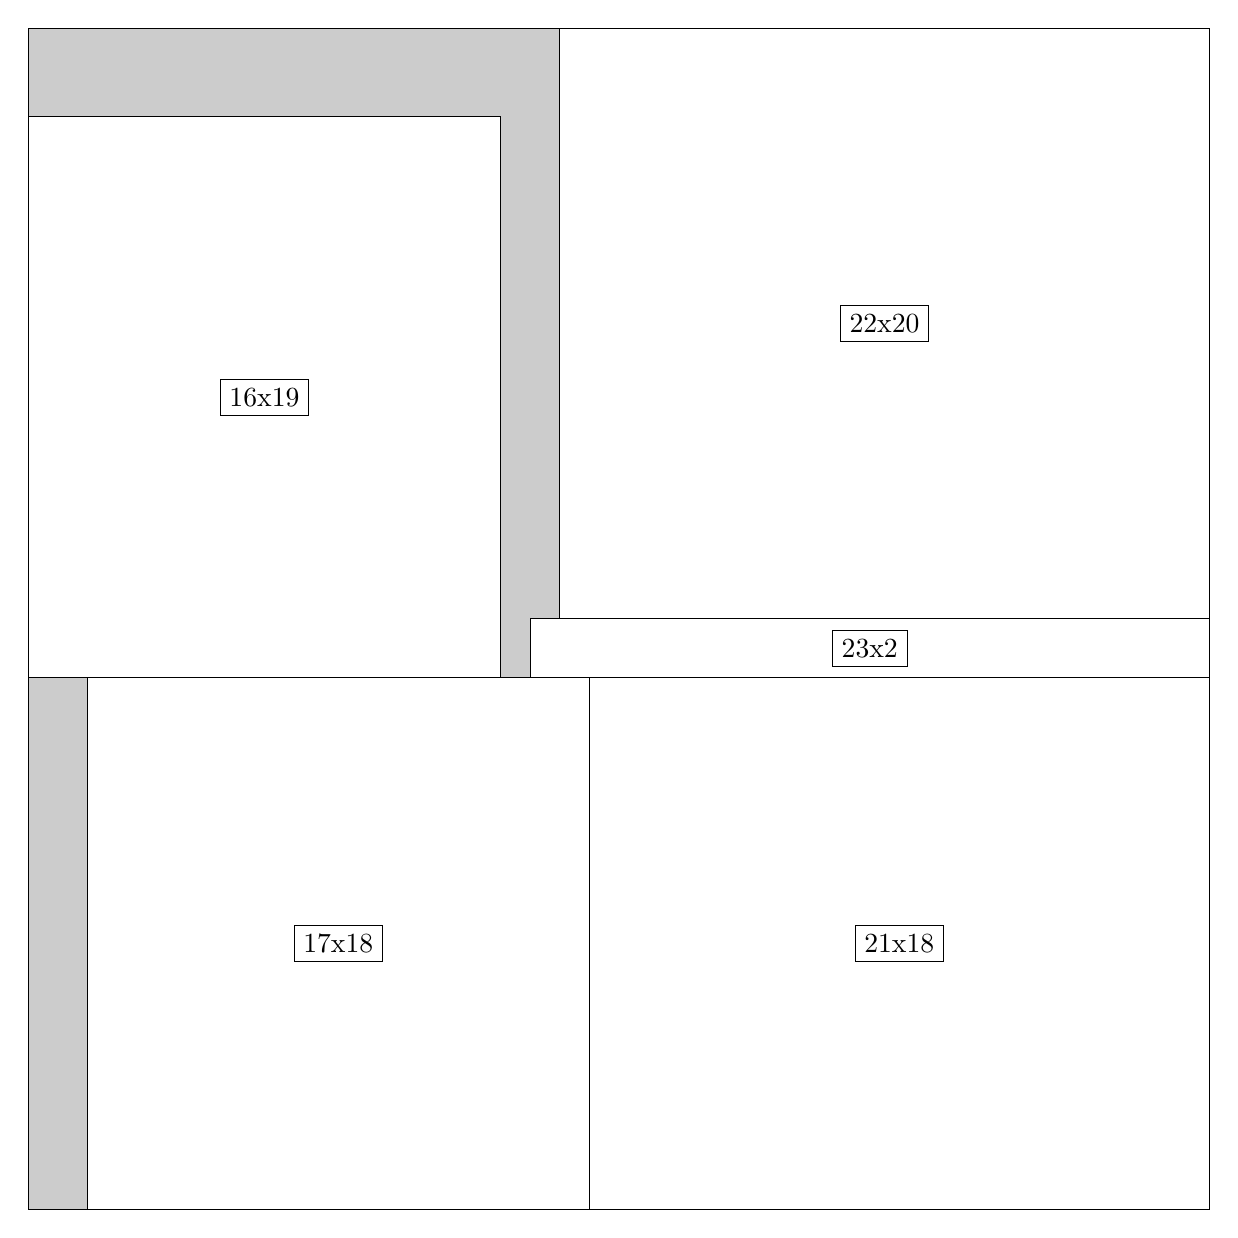
\begin{tikzpicture}[shorten >=1pt,scale=1.0,every node/.style={scale=1.0},->]
\tikzstyle{vertex}=[circle,fill=black!25,minimum size=14pt,inner sep=0pt]
\filldraw[fill=gray!40!white, draw=black] (0,0) rectangle (15.0,15.0);
\foreach \name/\x/\y/\w/\h in {21x18/7.125/0.0/7.875/6.75,17x18/0.75/0.0/6.375/6.75,23x2/6.375/6.75/8.625/0.75,22x20/6.75/7.5/8.25/7.5,16x19/0.0/6.75/6.0/7.125}
\filldraw[fill=white!40!white, draw=black] (\x,\y) rectangle node[draw] (\name) {\name} ++(\w,\h);
\end{tikzpicture}


w =21 , h =18 , x =19 , y =0 , v =378
\par
w =17 , h =18 , x =2 , y =0 , v =306
\par
w =23 , h =2 , x =17 , y =18 , v =46
\par
w =22 , h =20 , x =18 , y =20 , v =440
\par
w =16 , h =19 , x =0 , y =18 , v =304
\par
\newpage


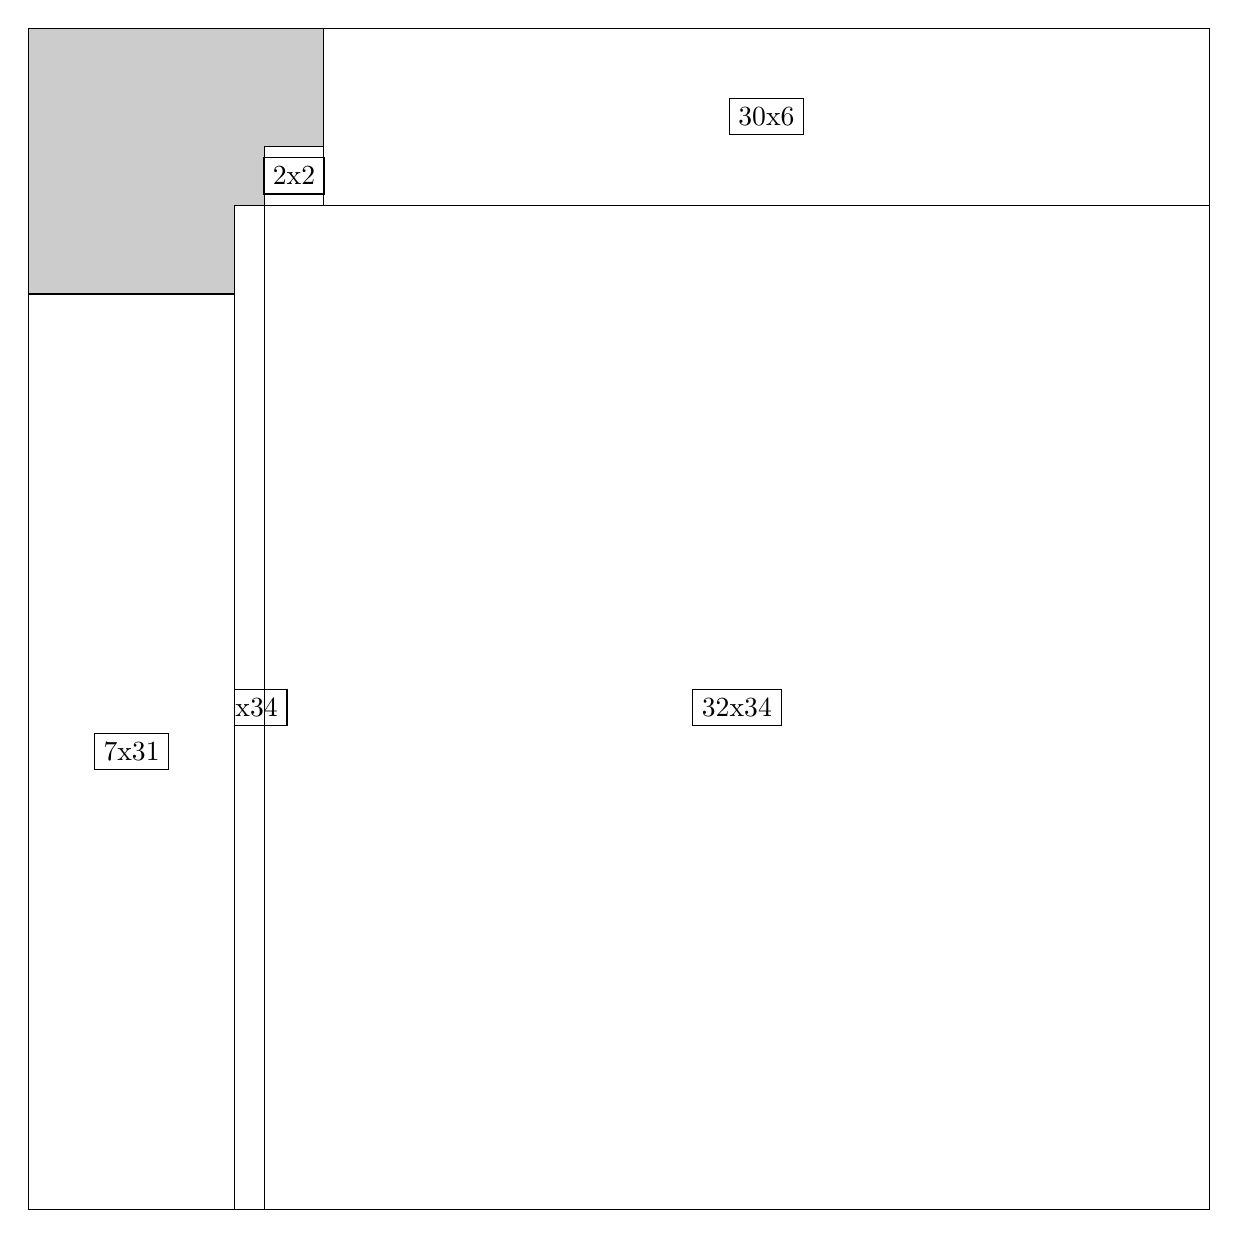
\begin{tikzpicture}[shorten >=1pt,scale=1.0,every node/.style={scale=1.0},->]
\tikzstyle{vertex}=[circle,fill=black!25,minimum size=14pt,inner sep=0pt]
\filldraw[fill=gray!40!white, draw=black] (0,0) rectangle (15.0,15.0);
\foreach \name/\x/\y/\w/\h in {32x34/3.0/0.0/12.0/12.75,30x6/3.75/12.75/11.25/2.25,2x2/3.0/12.75/0.75/0.75,1x34/2.625/0.0/0.375/12.75,7x31/0.0/0.0/2.625/11.625}
\filldraw[fill=white!40!white, draw=black] (\x,\y) rectangle node[draw] (\name) {\name} ++(\w,\h);
\end{tikzpicture}


w =32 , h =34 , x =8 , y =0 , v =1088
\par
w =30 , h =6 , x =10 , y =34 , v =180
\par
w =2 , h =2 , x =8 , y =34 , v =4
\par
w =1 , h =34 , x =7 , y =0 , v =34
\par
w =7 , h =31 , x =0 , y =0 , v =217
\par
\newpage


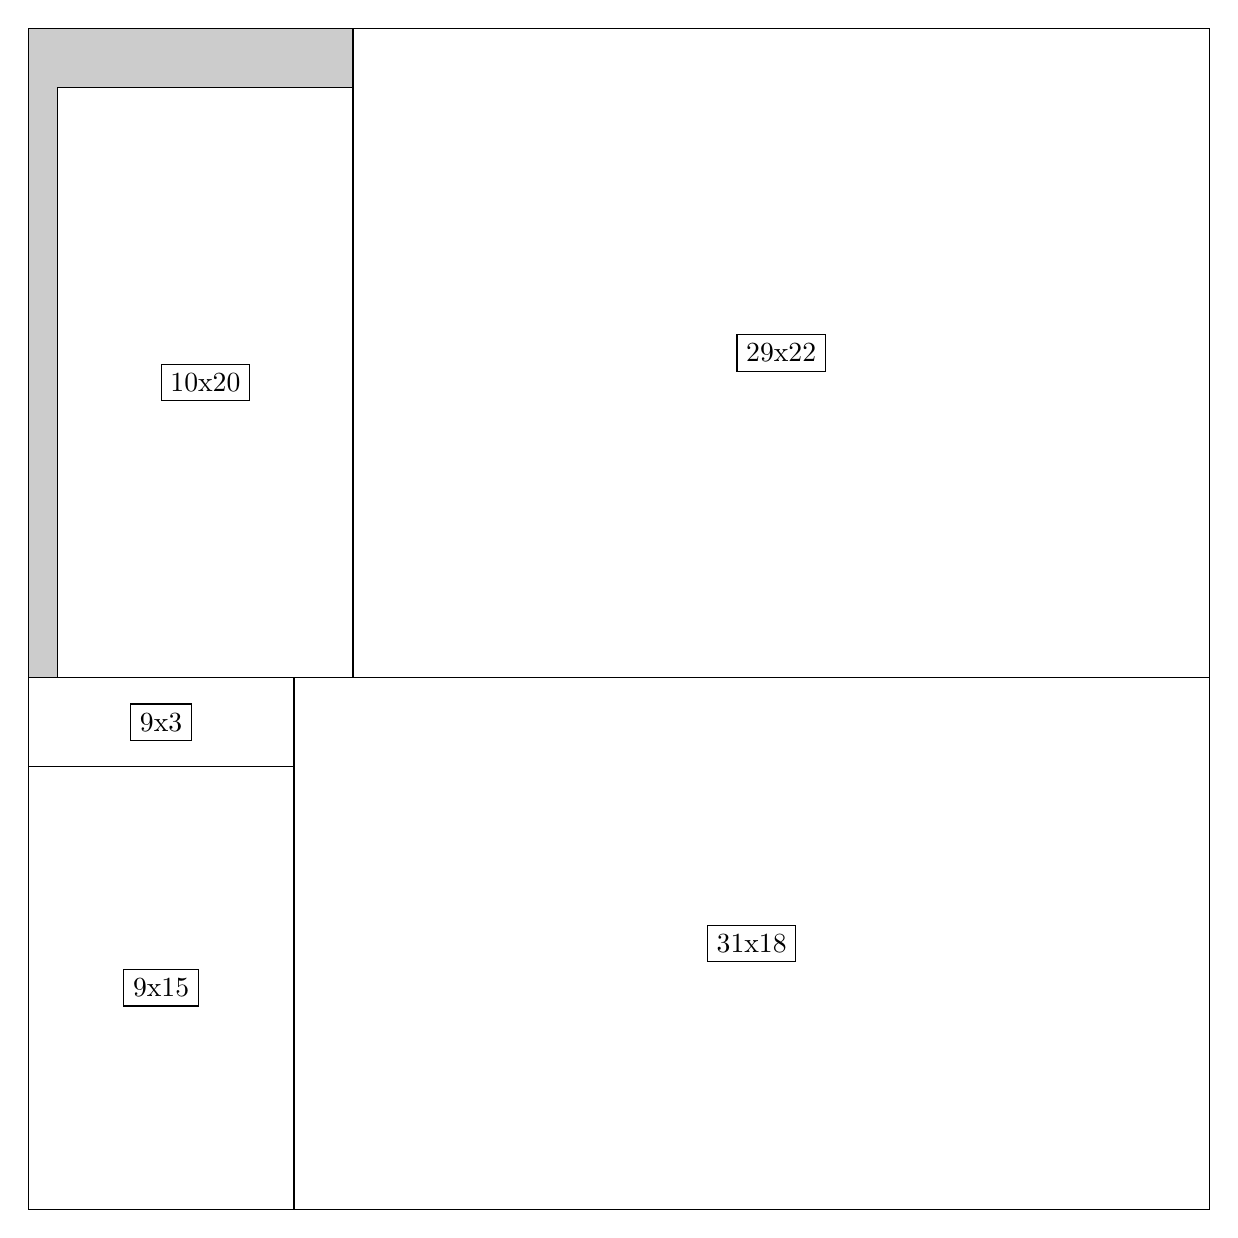
\begin{tikzpicture}[shorten >=1pt,scale=1.0,every node/.style={scale=1.0},->]
\tikzstyle{vertex}=[circle,fill=black!25,minimum size=14pt,inner sep=0pt]
\filldraw[fill=gray!40!white, draw=black] (0,0) rectangle (15.0,15.0);
\foreach \name/\x/\y/\w/\h in {31x18/3.375/0.0/11.625/6.75,9x15/0.0/0.0/3.375/5.625,9x3/0.0/5.625/3.375/1.125,29x22/4.125/6.75/10.875/8.25,10x20/0.375/6.75/3.75/7.5}
\filldraw[fill=white!40!white, draw=black] (\x,\y) rectangle node[draw] (\name) {\name} ++(\w,\h);
\end{tikzpicture}


w =31 , h =18 , x =9 , y =0 , v =558
\par
w =9 , h =15 , x =0 , y =0 , v =135
\par
w =9 , h =3 , x =0 , y =15 , v =27
\par
w =29 , h =22 , x =11 , y =18 , v =638
\par
w =10 , h =20 , x =1 , y =18 , v =200
\par
\newpage


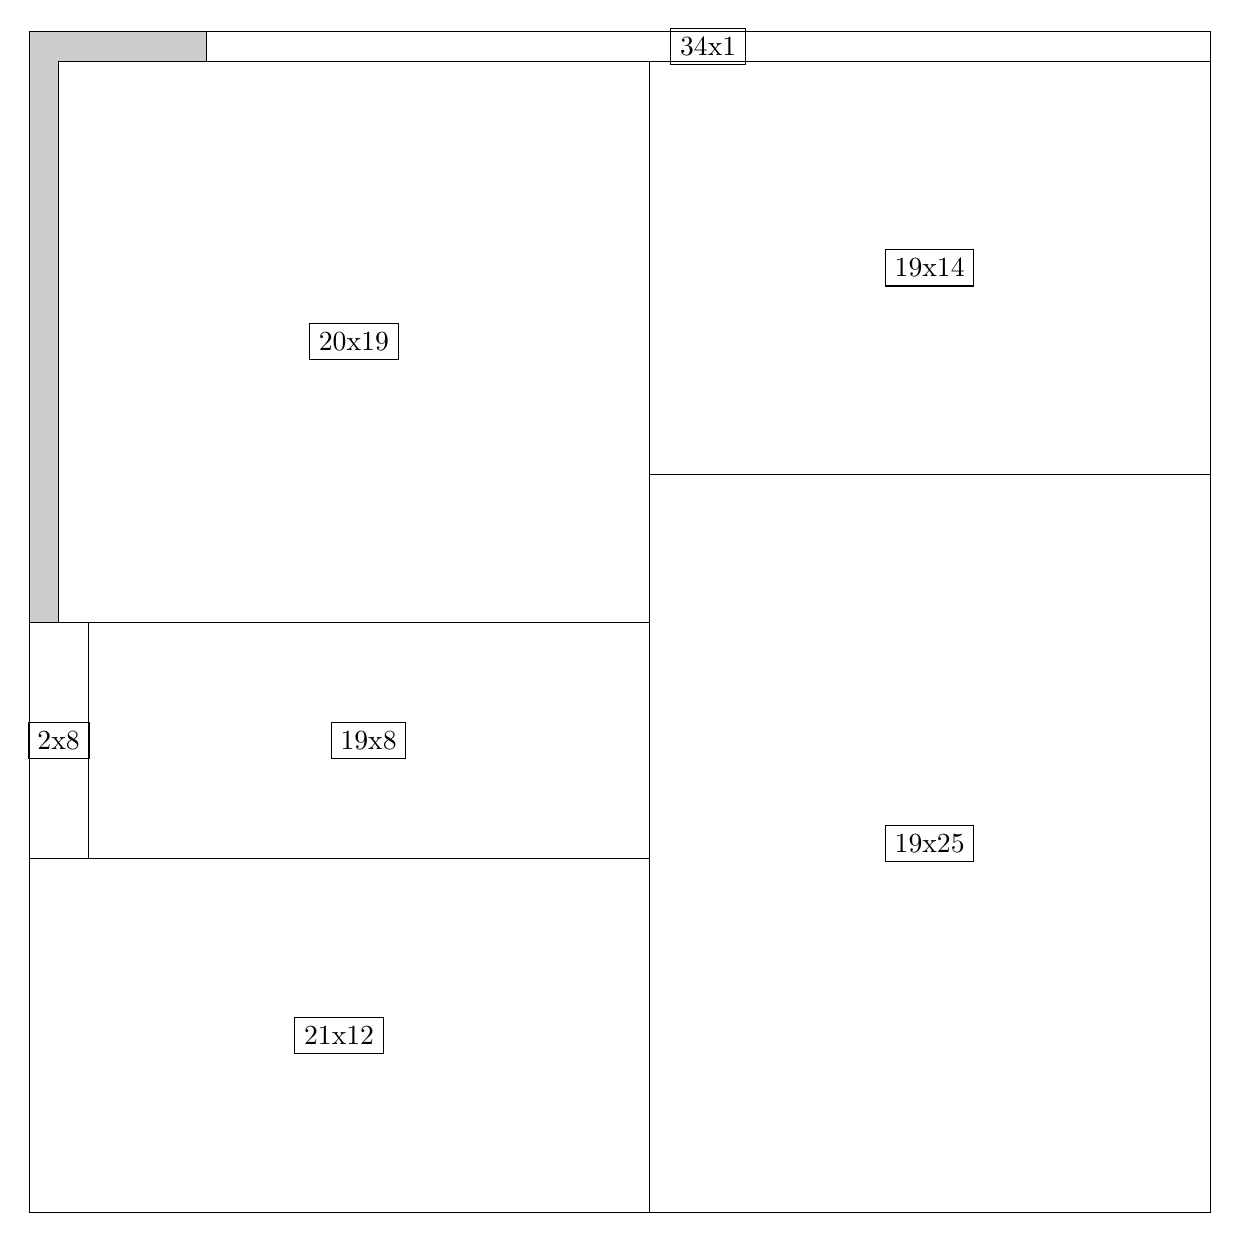
\begin{tikzpicture}[shorten >=1pt,scale=1.0,every node/.style={scale=1.0},->]
\tikzstyle{vertex}=[circle,fill=black!25,minimum size=14pt,inner sep=0pt]
\filldraw[fill=gray!40!white, draw=black] (0,0) rectangle (15.0,15.0);
\foreach \name/\x/\y/\w/\h in {19x25/7.875/0.0/7.125/9.375,19x14/7.875/9.375/7.125/5.25,21x12/0.0/0.0/7.875/4.5,19x8/0.75/4.5/7.125/3.0,2x8/0.0/4.5/0.75/3.0,20x19/0.375/7.5/7.5/7.125,34x1/2.25/14.625/12.75/0.375}
\filldraw[fill=white!40!white, draw=black] (\x,\y) rectangle node[draw] (\name) {\name} ++(\w,\h);
\end{tikzpicture}


w =19 , h =25 , x =21 , y =0 , v =475
\par
w =19 , h =14 , x =21 , y =25 , v =266
\par
w =21 , h =12 , x =0 , y =0 , v =252
\par
w =19 , h =8 , x =2 , y =12 , v =152
\par
w =2 , h =8 , x =0 , y =12 , v =16
\par
w =20 , h =19 , x =1 , y =20 , v =380
\par
w =34 , h =1 , x =6 , y =39 , v =34
\par
\newpage


\begin{tikzpicture}[shorten >=1pt,scale=1.0,every node/.style={scale=1.0},->]
\tikzstyle{vertex}=[circle,fill=black!25,minimum size=14pt,inner sep=0pt]
\filldraw[fill=gray!40!white, draw=black] (0,0) rectangle (15.0,15.0);
\foreach \name/\x/\y/\w/\h in {28x31/4.5/0.0/10.5/11.625,12x31/0.0/0.0/4.5/11.625,10x9/11.25/11.625/3.75/3.375,28x8/0.75/11.625/10.5/3.0,27x1/1.125/14.625/10.125/0.375}
\filldraw[fill=white!40!white, draw=black] (\x,\y) rectangle node[draw] (\name) {\name} ++(\w,\h);
\end{tikzpicture}


w =28 , h =31 , x =12 , y =0 , v =868
\par
w =12 , h =31 , x =0 , y =0 , v =372
\par
w =10 , h =9 , x =30 , y =31 , v =90
\par
w =28 , h =8 , x =2 , y =31 , v =224
\par
w =27 , h =1 , x =3 , y =39 , v =27
\par
\newpage


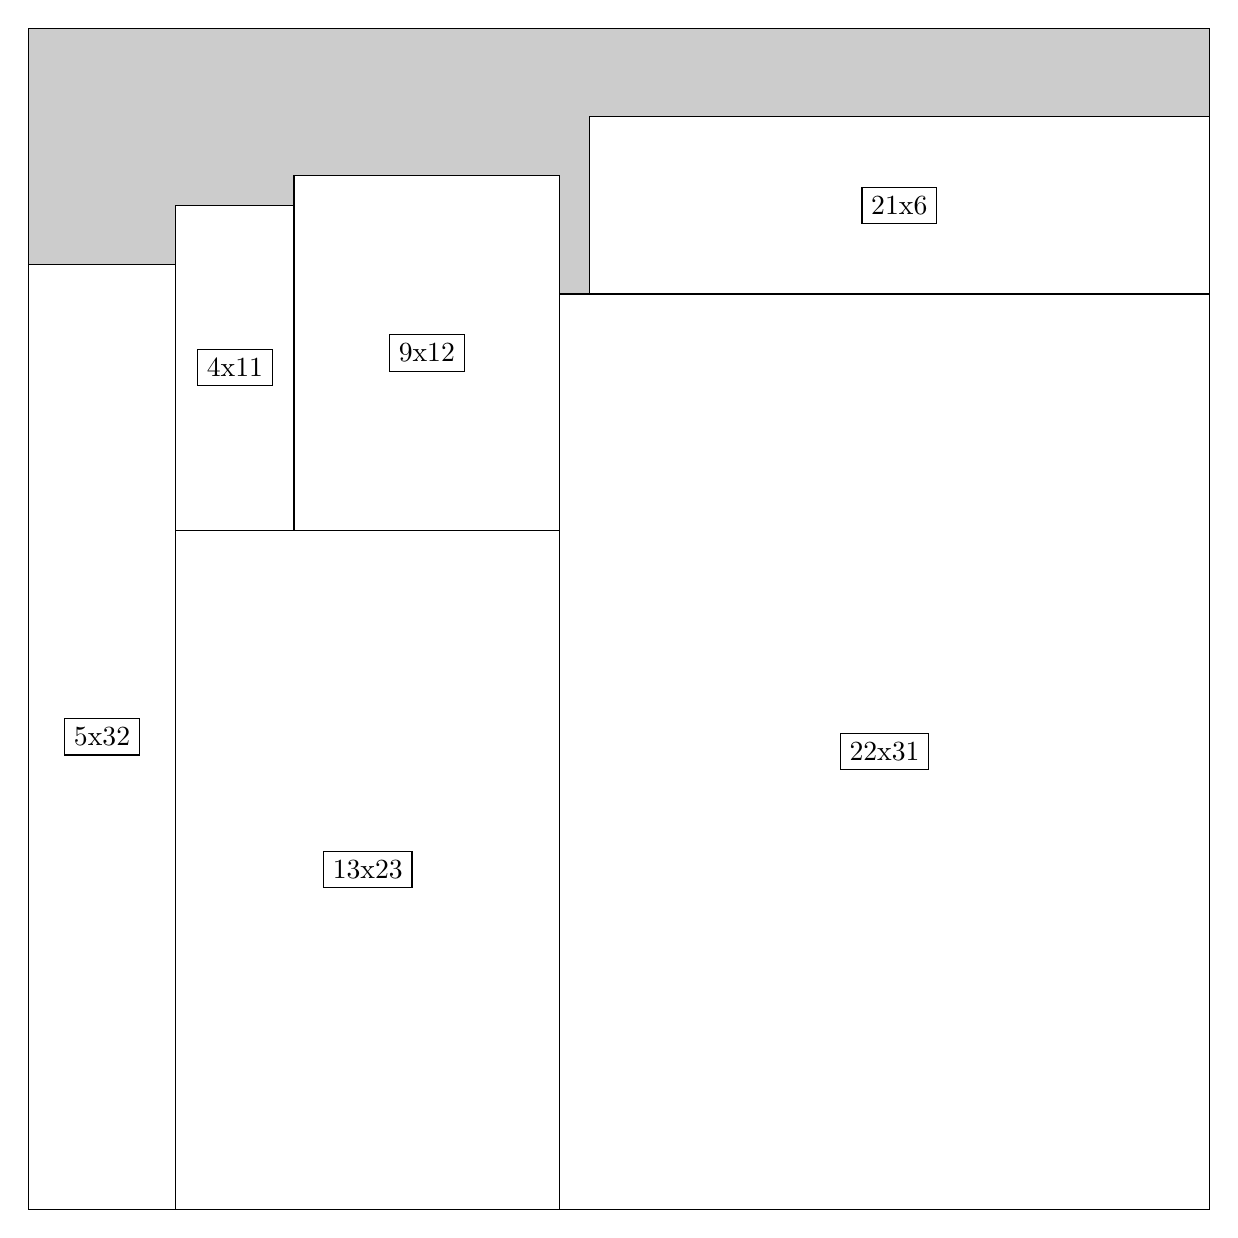
\begin{tikzpicture}[shorten >=1pt,scale=1.0,every node/.style={scale=1.0},->]
\tikzstyle{vertex}=[circle,fill=black!25,minimum size=14pt,inner sep=0pt]
\filldraw[fill=gray!40!white, draw=black] (0,0) rectangle (15.0,15.0);
\foreach \name/\x/\y/\w/\h in {22x31/6.75/0.0/8.25/11.625,21x6/7.125/11.625/7.875/2.25,13x23/1.875/0.0/4.875/8.625,9x12/3.375/8.625/3.375/4.5,4x11/1.875/8.625/1.5/4.125,5x32/0.0/0.0/1.875/12.0}
\filldraw[fill=white!40!white, draw=black] (\x,\y) rectangle node[draw] (\name) {\name} ++(\w,\h);
\end{tikzpicture}


w =22 , h =31 , x =18 , y =0 , v =682
\par
w =21 , h =6 , x =19 , y =31 , v =126
\par
w =13 , h =23 , x =5 , y =0 , v =299
\par
w =9 , h =12 , x =9 , y =23 , v =108
\par
w =4 , h =11 , x =5 , y =23 , v =44
\par
w =5 , h =32 , x =0 , y =0 , v =160
\par
\newpage


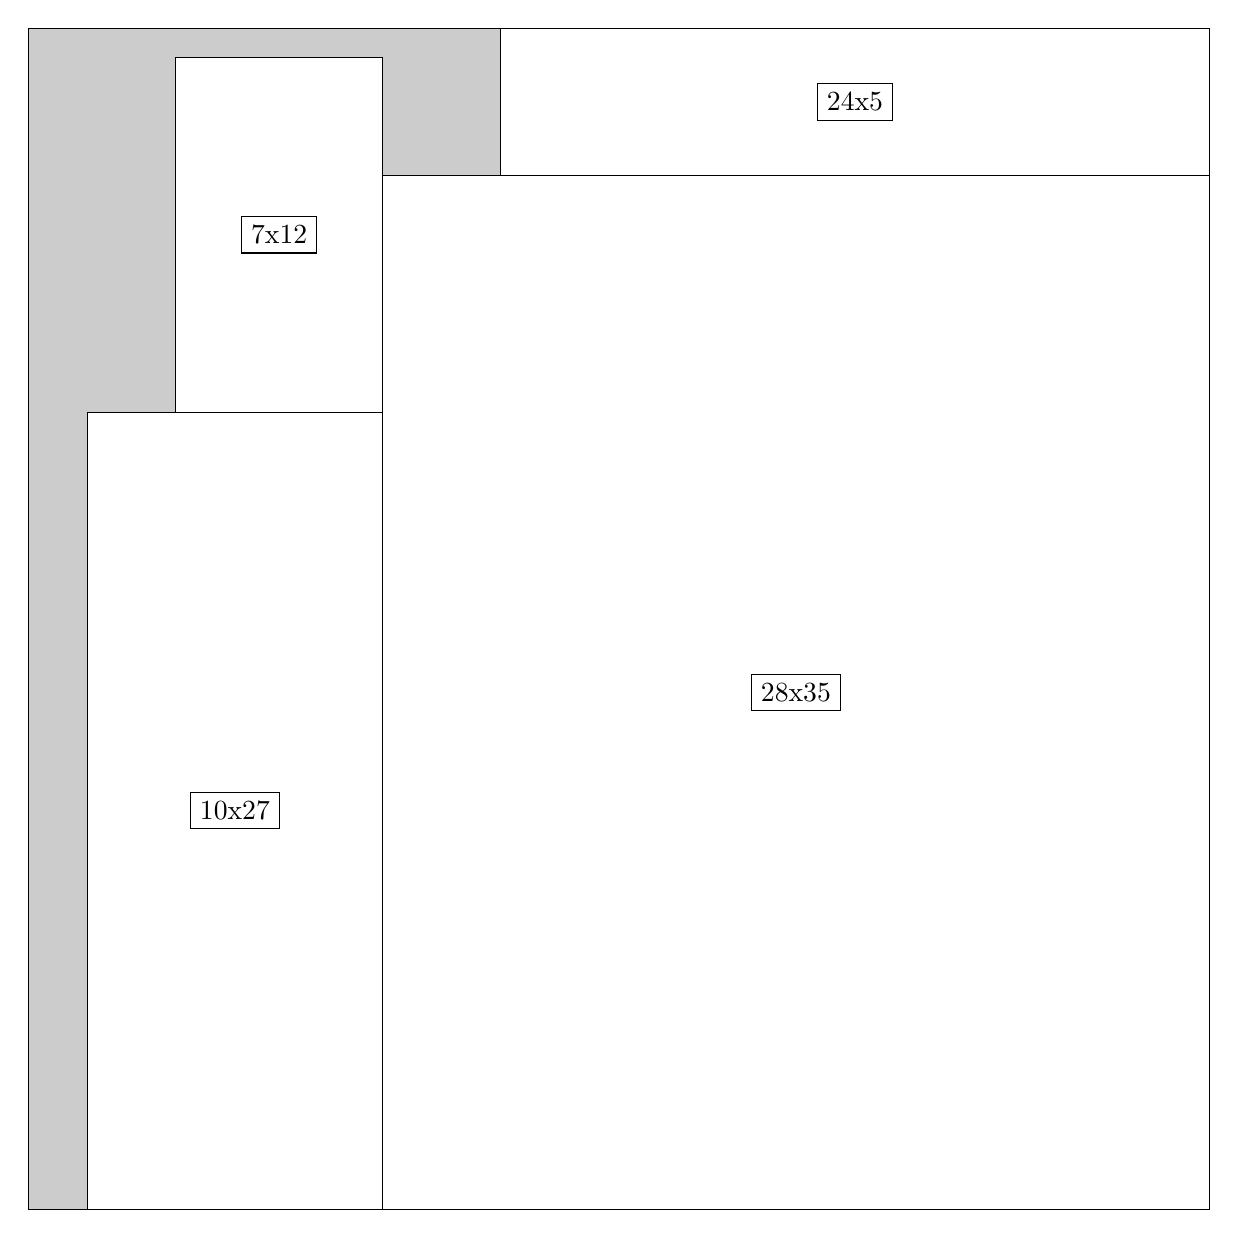
\begin{tikzpicture}[shorten >=1pt,scale=1.0,every node/.style={scale=1.0},->]
\tikzstyle{vertex}=[circle,fill=black!25,minimum size=14pt,inner sep=0pt]
\filldraw[fill=gray!40!white, draw=black] (0,0) rectangle (15.0,15.0);
\foreach \name/\x/\y/\w/\h in {28x35/4.5/0.0/10.5/13.125,24x5/6.0/13.125/9.0/1.875,10x27/0.75/0.0/3.75/10.125,7x12/1.875/10.125/2.625/4.5}
\filldraw[fill=white!40!white, draw=black] (\x,\y) rectangle node[draw] (\name) {\name} ++(\w,\h);
\end{tikzpicture}


w =28 , h =35 , x =12 , y =0 , v =980
\par
w =24 , h =5 , x =16 , y =35 , v =120
\par
w =10 , h =27 , x =2 , y =0 , v =270
\par
w =7 , h =12 , x =5 , y =27 , v =84
\par
\newpage


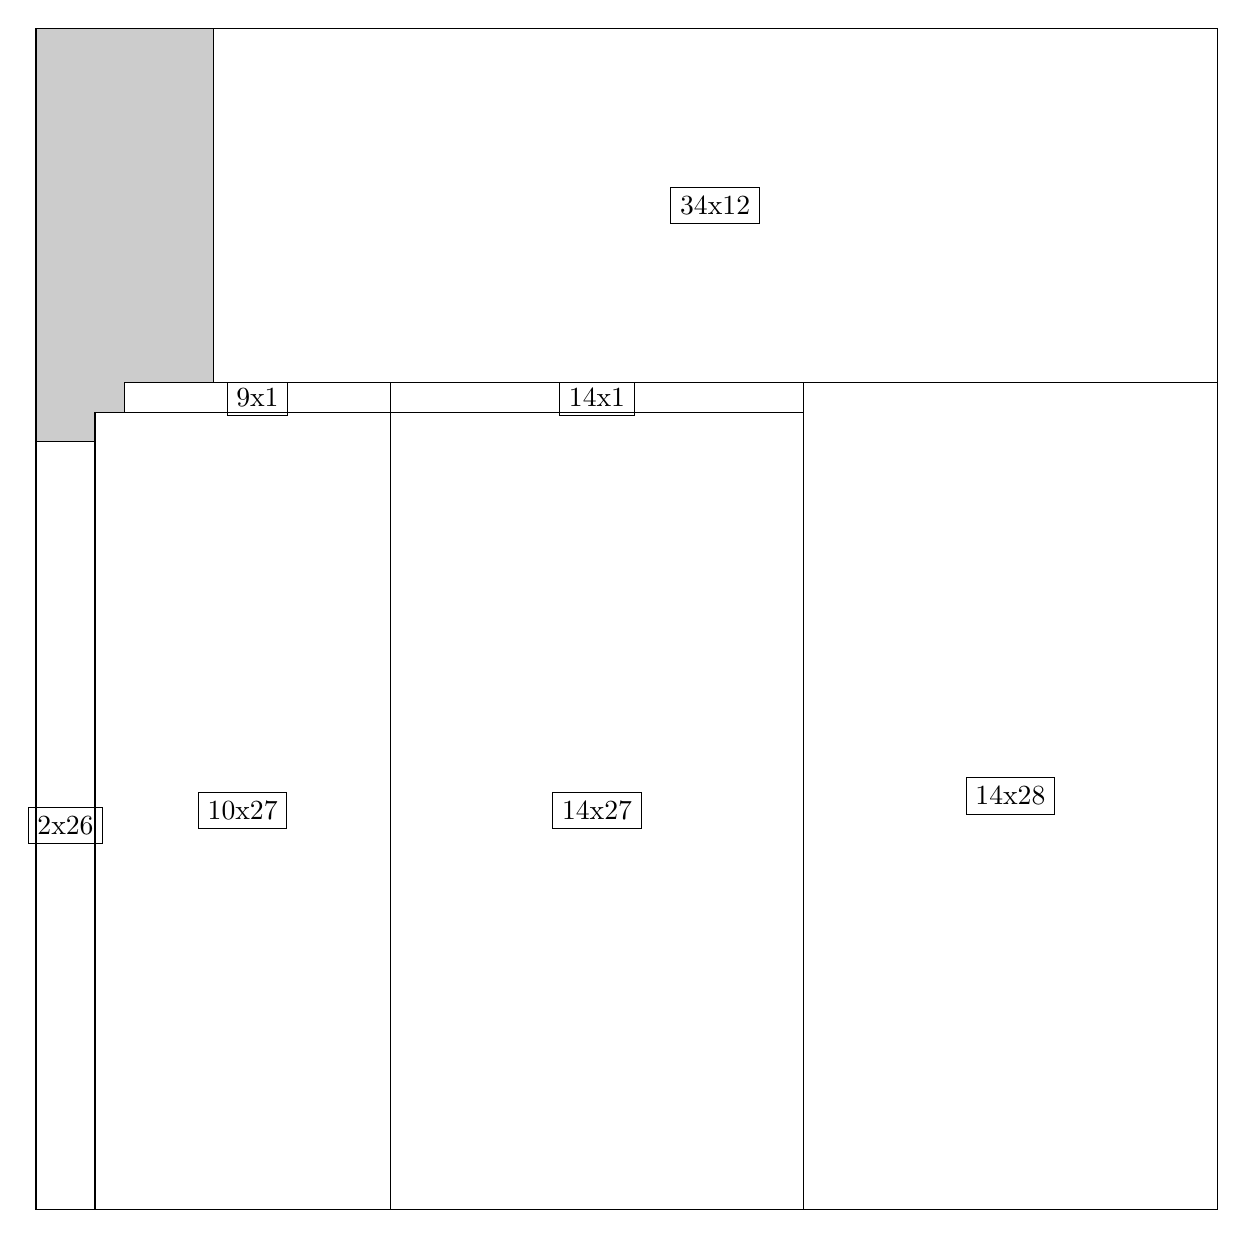
\begin{tikzpicture}[shorten >=1pt,scale=1.0,every node/.style={scale=1.0},->]
\tikzstyle{vertex}=[circle,fill=black!25,minimum size=14pt,inner sep=0pt]
\filldraw[fill=gray!40!white, draw=black] (0,0) rectangle (15.0,15.0);
\foreach \name/\x/\y/\w/\h in {14x28/9.75/0.0/5.25/10.5,14x27/4.5/0.0/5.25/10.125,14x1/4.5/10.125/5.25/0.375,10x27/0.75/0.0/3.75/10.125,9x1/1.125/10.125/3.375/0.375,2x26/0.0/0.0/0.75/9.75,34x12/2.25/10.5/12.75/4.5}
\filldraw[fill=white!40!white, draw=black] (\x,\y) rectangle node[draw] (\name) {\name} ++(\w,\h);
\end{tikzpicture}


w =14 , h =28 , x =26 , y =0 , v =392
\par
w =14 , h =27 , x =12 , y =0 , v =378
\par
w =14 , h =1 , x =12 , y =27 , v =14
\par
w =10 , h =27 , x =2 , y =0 , v =270
\par
w =9 , h =1 , x =3 , y =27 , v =9
\par
w =2 , h =26 , x =0 , y =0 , v =52
\par
w =34 , h =12 , x =6 , y =28 , v =408
\par
\newpage


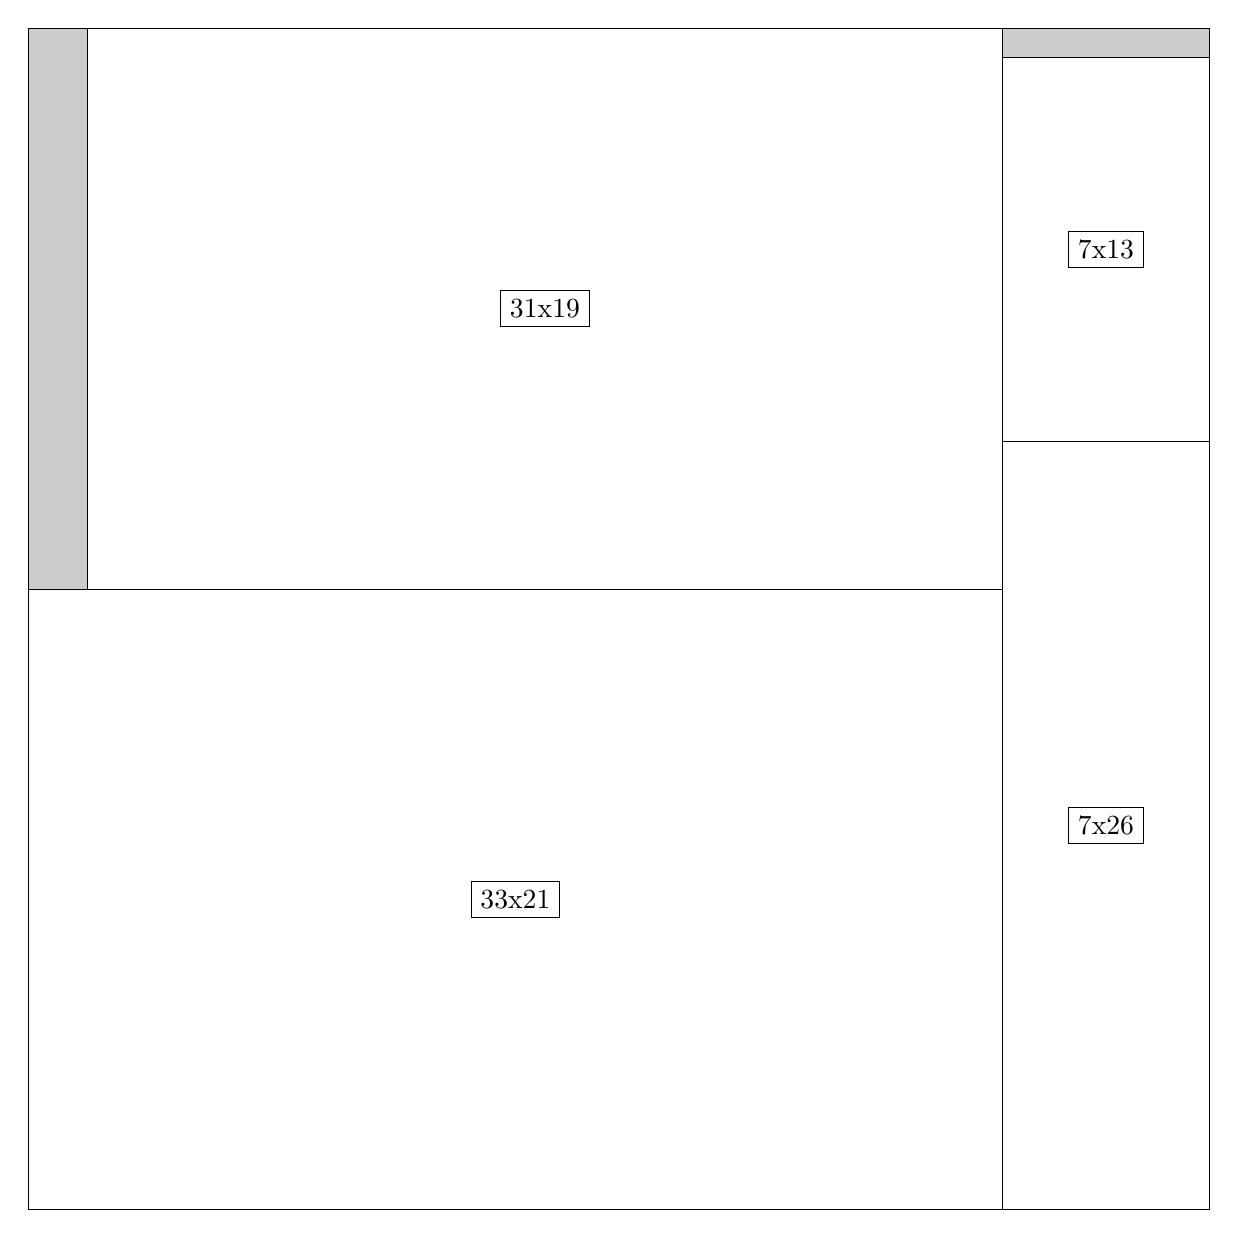
\begin{tikzpicture}[shorten >=1pt,scale=1.0,every node/.style={scale=1.0},->]
\tikzstyle{vertex}=[circle,fill=black!25,minimum size=14pt,inner sep=0pt]
\filldraw[fill=gray!40!white, draw=black] (0,0) rectangle (15.0,15.0);
\foreach \name/\x/\y/\w/\h in {7x26/12.375/0.0/2.625/9.75,7x13/12.375/9.75/2.625/4.875,33x21/0.0/0.0/12.375/7.875,31x19/0.75/7.875/11.625/7.125}
\filldraw[fill=white!40!white, draw=black] (\x,\y) rectangle node[draw] (\name) {\name} ++(\w,\h);
\end{tikzpicture}


w =7 , h =26 , x =33 , y =0 , v =182
\par
w =7 , h =13 , x =33 , y =26 , v =91
\par
w =33 , h =21 , x =0 , y =0 , v =693
\par
w =31 , h =19 , x =2 , y =21 , v =589
\par
\newpage


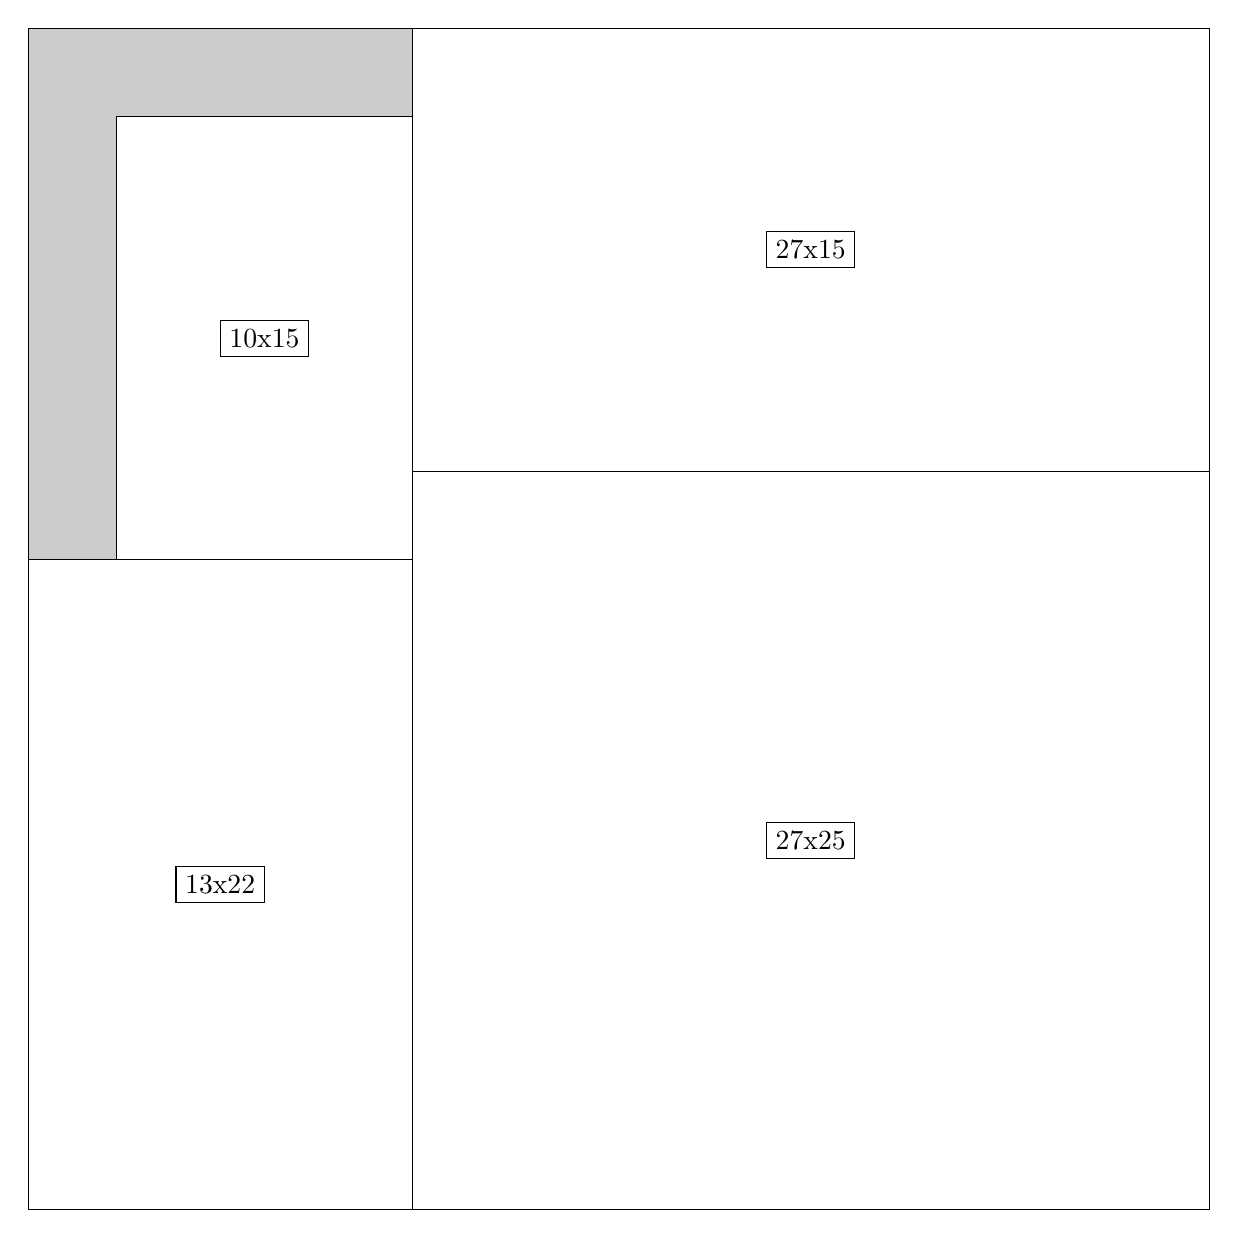
\begin{tikzpicture}[shorten >=1pt,scale=1.0,every node/.style={scale=1.0},->]
\tikzstyle{vertex}=[circle,fill=black!25,minimum size=14pt,inner sep=0pt]
\filldraw[fill=gray!40!white, draw=black] (0,0) rectangle (15.0,15.0);
\foreach \name/\x/\y/\w/\h in {27x25/4.875/0.0/10.125/9.375,27x15/4.875/9.375/10.125/5.625,13x22/0.0/0.0/4.875/8.25,10x15/1.125/8.25/3.75/5.625}
\filldraw[fill=white!40!white, draw=black] (\x,\y) rectangle node[draw] (\name) {\name} ++(\w,\h);
\end{tikzpicture}


w =27 , h =25 , x =13 , y =0 , v =675
\par
w =27 , h =15 , x =13 , y =25 , v =405
\par
w =13 , h =22 , x =0 , y =0 , v =286
\par
w =10 , h =15 , x =3 , y =22 , v =150
\par
\newpage


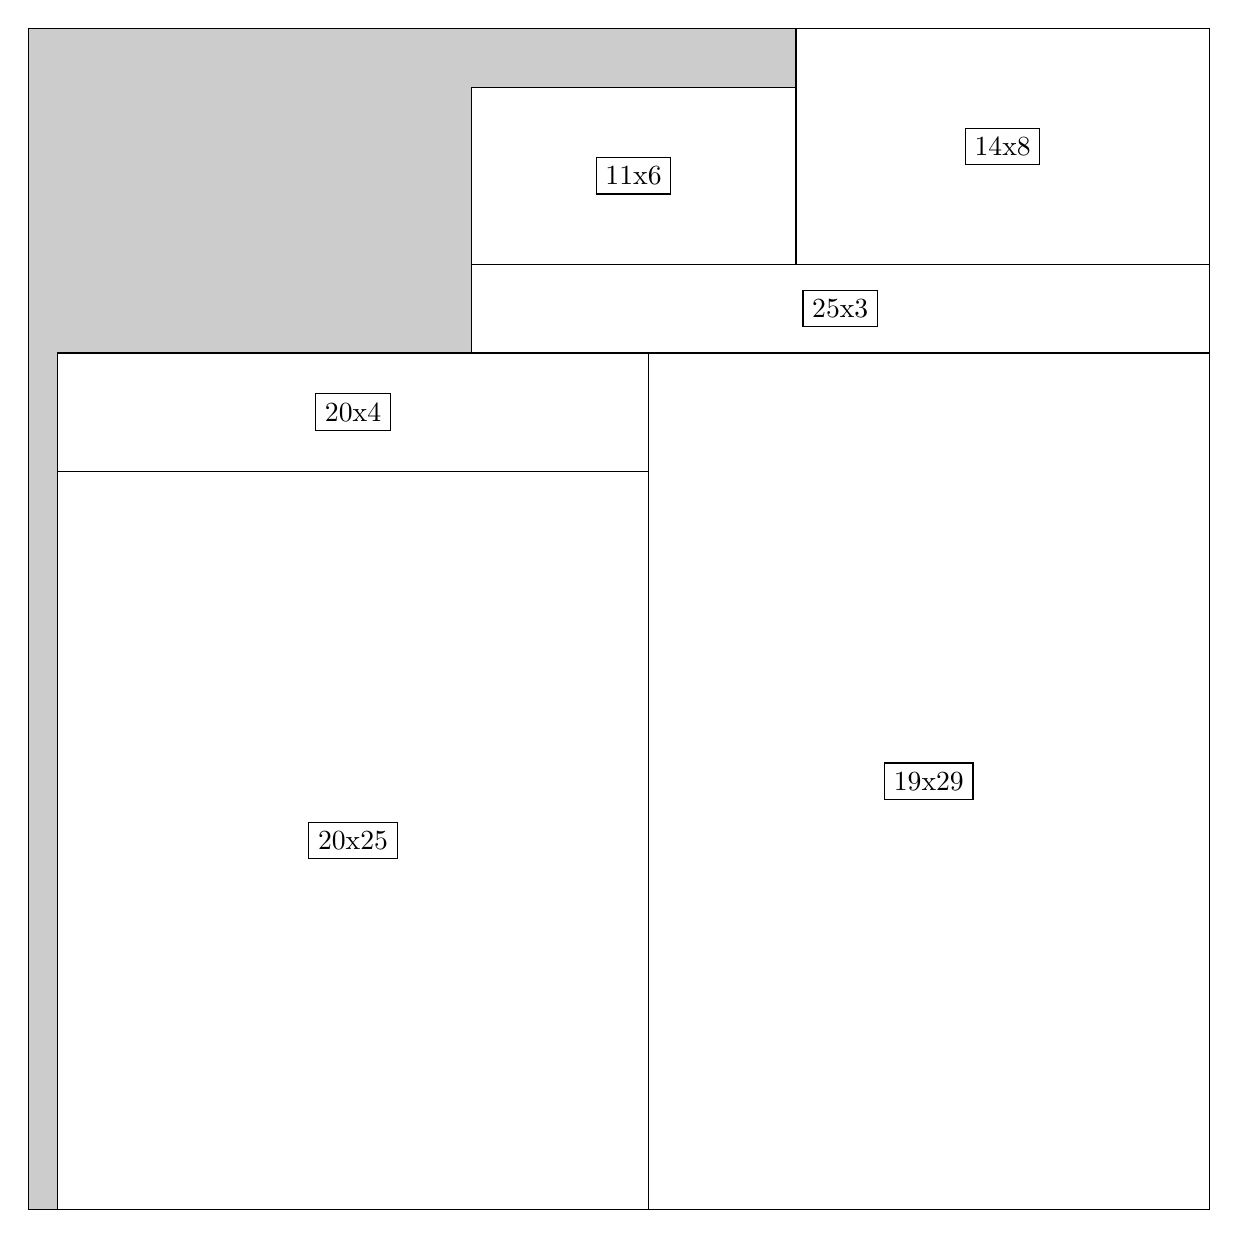
\begin{tikzpicture}[shorten >=1pt,scale=1.0,every node/.style={scale=1.0},->]
\tikzstyle{vertex}=[circle,fill=black!25,minimum size=14pt,inner sep=0pt]
\filldraw[fill=gray!40!white, draw=black] (0,0) rectangle (15.0,15.0);
\foreach \name/\x/\y/\w/\h in {19x29/7.875/0.0/7.125/10.875,20x25/0.375/0.0/7.5/9.375,20x4/0.375/9.375/7.5/1.5,25x3/5.625/10.875/9.375/1.125,14x8/9.75/12.0/5.25/3.0,11x6/5.625/12.0/4.125/2.25}
\filldraw[fill=white!40!white, draw=black] (\x,\y) rectangle node[draw] (\name) {\name} ++(\w,\h);
\end{tikzpicture}


w =19 , h =29 , x =21 , y =0 , v =551
\par
w =20 , h =25 , x =1 , y =0 , v =500
\par
w =20 , h =4 , x =1 , y =25 , v =80
\par
w =25 , h =3 , x =15 , y =29 , v =75
\par
w =14 , h =8 , x =26 , y =32 , v =112
\par
w =11 , h =6 , x =15 , y =32 , v =66
\par
\newpage


\begin{tikzpicture}[shorten >=1pt,scale=1.0,every node/.style={scale=1.0},->]
\tikzstyle{vertex}=[circle,fill=black!25,minimum size=14pt,inner sep=0pt]
\filldraw[fill=gray!40!white, draw=black] (0,0) rectangle (15.0,15.0);
\foreach \name/\x/\y/\w/\h in {26x28/5.25/0.0/9.75/10.5,14x28/0.0/0.0/5.25/10.5,35x12/1.875/10.5/13.125/4.5,5x11/0.0/10.5/1.875/4.125}
\filldraw[fill=white!40!white, draw=black] (\x,\y) rectangle node[draw] (\name) {\name} ++(\w,\h);
\end{tikzpicture}


w =26 , h =28 , x =14 , y =0 , v =728
\par
w =14 , h =28 , x =0 , y =0 , v =392
\par
w =35 , h =12 , x =5 , y =28 , v =420
\par
w =5 , h =11 , x =0 , y =28 , v =55
\par
\newpage


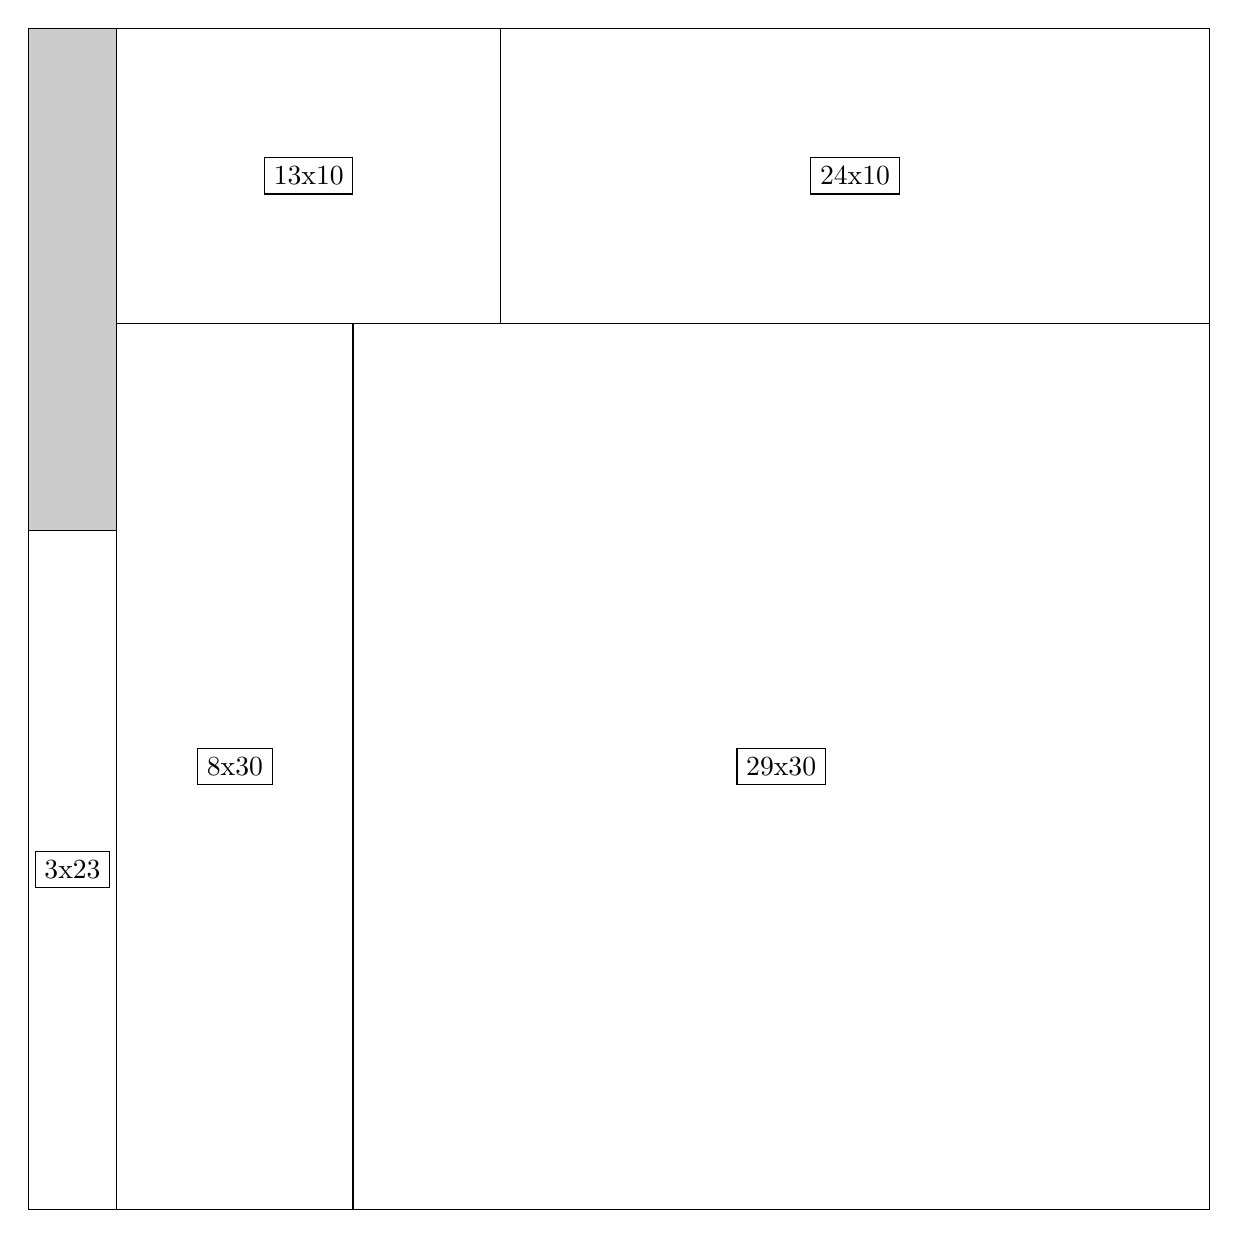
\begin{tikzpicture}[shorten >=1pt,scale=1.0,every node/.style={scale=1.0},->]
\tikzstyle{vertex}=[circle,fill=black!25,minimum size=14pt,inner sep=0pt]
\filldraw[fill=gray!40!white, draw=black] (0,0) rectangle (15.0,15.0);
\foreach \name/\x/\y/\w/\h in {29x30/4.125/0.0/10.875/11.25,8x30/1.125/0.0/3.0/11.25,3x23/0.0/0.0/1.125/8.625,24x10/6.0/11.25/9.0/3.75,13x10/1.125/11.25/4.875/3.75}
\filldraw[fill=white!40!white, draw=black] (\x,\y) rectangle node[draw] (\name) {\name} ++(\w,\h);
\end{tikzpicture}


w =29 , h =30 , x =11 , y =0 , v =870
\par
w =8 , h =30 , x =3 , y =0 , v =240
\par
w =3 , h =23 , x =0 , y =0 , v =69
\par
w =24 , h =10 , x =16 , y =30 , v =240
\par
w =13 , h =10 , x =3 , y =30 , v =130
\par
\newpage


\begin{tikzpicture}[shorten >=1pt,scale=1.0,every node/.style={scale=1.0},->]
\tikzstyle{vertex}=[circle,fill=black!25,minimum size=14pt,inner sep=0pt]
\filldraw[fill=gray!40!white, draw=black] (0,0) rectangle (15.0,15.0);
\foreach \name/\x/\y/\w/\h in {18x27/8.25/0.0/6.75/10.125,18x13/8.25/10.125/6.75/4.875,22x33/0.0/0.0/8.25/12.375,22x6/0.0/12.375/8.25/2.25}
\filldraw[fill=white!40!white, draw=black] (\x,\y) rectangle node[draw] (\name) {\name} ++(\w,\h);
\end{tikzpicture}


w =18 , h =27 , x =22 , y =0 , v =486
\par
w =18 , h =13 , x =22 , y =27 , v =234
\par
w =22 , h =33 , x =0 , y =0 , v =726
\par
w =22 , h =6 , x =0 , y =33 , v =132
\par
\newpage


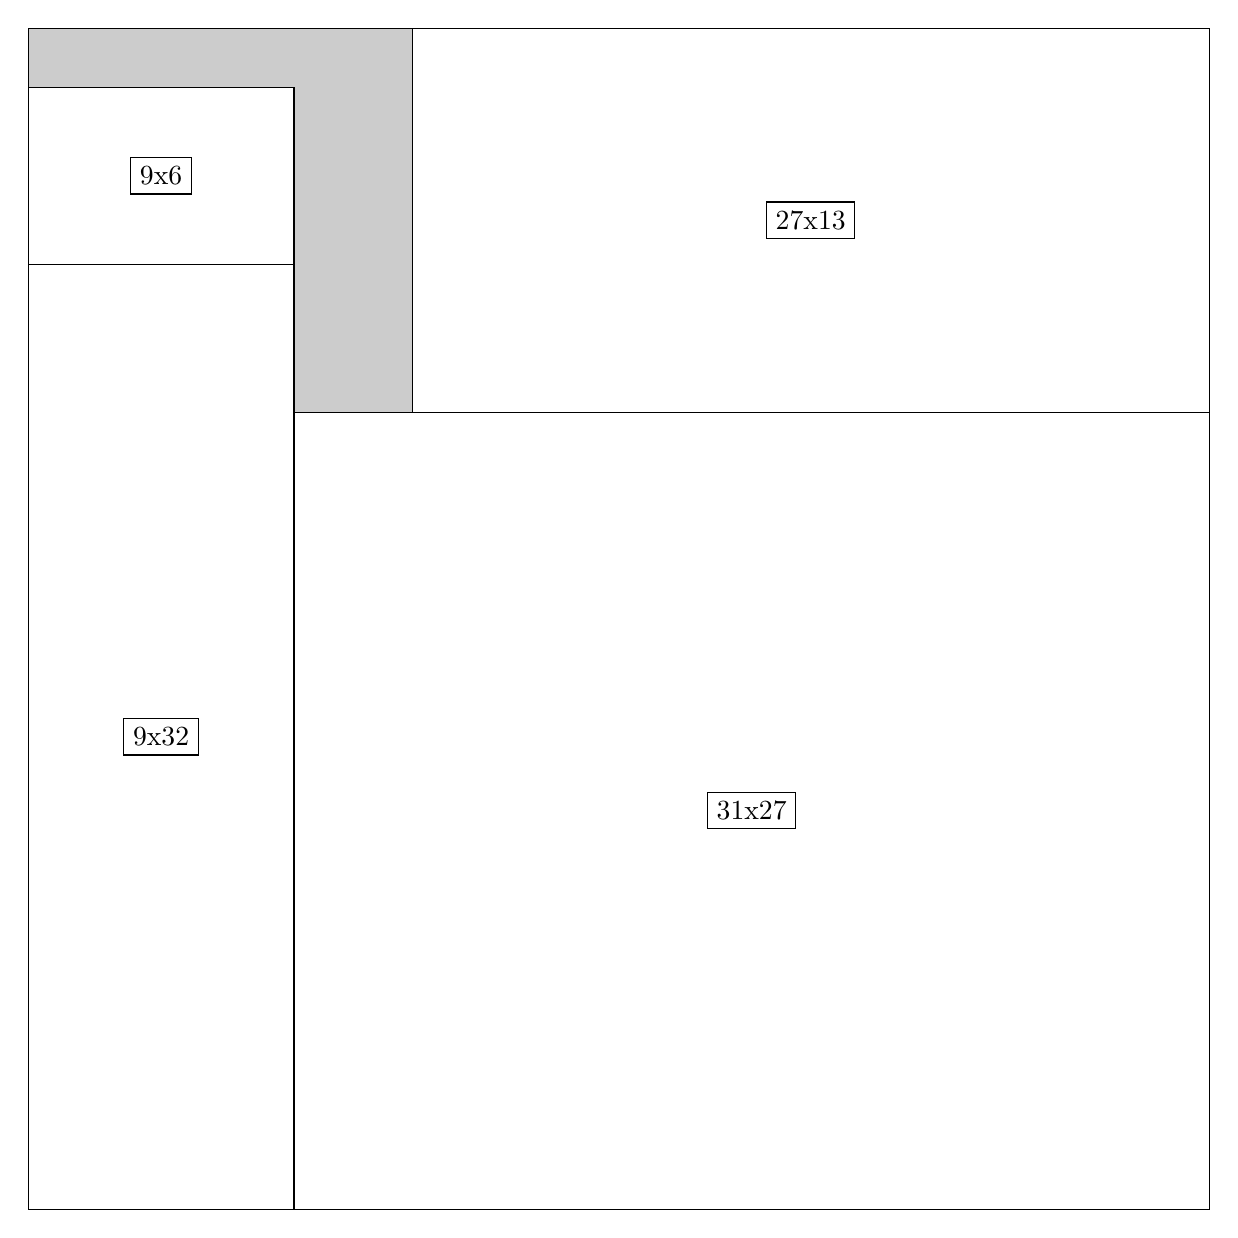
\begin{tikzpicture}[shorten >=1pt,scale=1.0,every node/.style={scale=1.0},->]
\tikzstyle{vertex}=[circle,fill=black!25,minimum size=14pt,inner sep=0pt]
\filldraw[fill=gray!40!white, draw=black] (0,0) rectangle (15.0,15.0);
\foreach \name/\x/\y/\w/\h in {31x27/3.375/0.0/11.625/10.125,27x13/4.875/10.125/10.125/4.875,9x32/0.0/0.0/3.375/12.0,9x6/0.0/12.0/3.375/2.25}
\filldraw[fill=white!40!white, draw=black] (\x,\y) rectangle node[draw] (\name) {\name} ++(\w,\h);
\end{tikzpicture}


w =31 , h =27 , x =9 , y =0 , v =837
\par
w =27 , h =13 , x =13 , y =27 , v =351
\par
w =9 , h =32 , x =0 , y =0 , v =288
\par
w =9 , h =6 , x =0 , y =32 , v =54
\par
\newpage


\end{document}